% Evolutionary Computing, Standard Assignment, Task II (neuroevolution).
% GECCO'19 template (ACM sigconf, from the course's latex_template.zip).
% Limit: 6 pages, excluding the cover page and the bibliography.
% Every number here comes from the repository: docs/decisions.md (Dx),
% experiments/README.md, results/olympic/analysis/summary.md and
% results/olympic/probabilities*.md. Search for \todo before submitting.
\documentclass[sigconf]{acmart}

\usepackage{booktabs}
\usepackage{xcolor}
\usepackage{amsmath}
\usepackage{tabularx}

% No ACM copyright block, reference format or running conference header.
\settopmatter{printacmref=false, printccs=false, printfolios=true}
\setcopyright{none}
\renewcommand\footnotetextcopyrightpermission[1]{}
\acmConference{}{}{}
\acmDOI{}
\acmISBN{}
\acmPrice{}
\pagestyle{plain}

\newcommand{\todo}[1]{\textcolor{red}{[TODO: #1]}}
% A figure that may not exist yet: a framed placeholder until it does.
\newcommand{\maybegraphic}[2]{%
  \IfFileExists{#2}{\includegraphics[width=#1]{#2}}{%
    \fbox{\parbox{#1}{\centering\vspace{1.5cm}\texttt{#2} (run paper\_figures.py)\vspace{1.5cm}}}}}

\begin{document}

% ---------------------------------------------------------------- cover page
\begin{titlepage}
  \centering
  \vspace*{3cm}
  {\Large Evolutionary Computing (X\_400111)\par}
  \vspace{0.6cm}
  {\large Standard Assignment, Task II: Neuroevolution\par}
  \vspace{1.6cm}
  {\LARGE\bfseries Send the Best, the Worst, or Anyone?\par}
  \vspace{0.3cm}
  {\Large Emigrant Selection in Island-Model Neuroevolution\\ of a Walking Robot\par}
  \vspace{1.6cm}
  {\large Team 92 \todo{confirm the A2 team number}\par}
  \vspace{0.8cm}
  \begin{tabular}{ll}
    Mehmet Emre Ozkan & 2933667 \\
    Wiktoria Popko    & 2938109 \\
    Manisha Venkatesha & 2922492 \\
    Anshul Rao        & 2914098 \\
  \end{tabular}
  \todo{confirm the team members}\par
  \vfill
  {\large \todo{submission date}, October 2026\par}
  \vspace{1cm}
  Vrije Universiteit Amsterdam
\end{titlepage}

% ------------------------------------------------------------------ the paper
\title{Send the Best, the Worst, or Anyone? Emigrant Selection in Island-Model
Neuroevolution of a Walking Robot}

\author{Mehmet Emre Ozkan}
\affiliation{\institution{2933667}}
\author{Wiktoria Popko}
\affiliation{\institution{2938109}}
\author{Manisha Venkatesha}
\affiliation{\institution{2922492}}
\author{Anshul Rao}
\affiliation{\institution{2914098}}
\renewcommand{\shortauthors}{Ozkan, Popko, Venkatesha and Rao}

\begin{abstract}
We evolve the 212 weights of a 16-8-4-8 neural network that makes the
eight-hinge \texttt{spider\_8} robot of the ARIEL framework walk 2\,m to a
target on the OlympicArena within 15\,s. Our research question is how the
emigrant-selection policy of a four-island ring model (migrating the best,
the worst or random individuals, or not migrating at all) affects the speed and
the outcome of evolution. Over five paired seeds of 12{,}000 evaluations each,
every evolutionary algorithm beats random search (final fitness 0.96--1.25
against 2.60). Migration of any kind speeds up convergence compared with
isolated islands (posterior probability 89--96\% on the area under the
convergence curve), and migrating the best is the fastest: it reached a
fitness of 1.6 after 2{,}906 evaluations on average, against 5{,}466 without
migration. The final fitness and the performance on 20 unseen arenas, however,
do not depend measurably on the policy, and a single panmictic population was
as fast and ended best. A follow-up shows that \emph{how often} the islands
migrate matters more than \emph{whom} they send: every 5--20 generations is
equally fast, every 50 is as slow as no migration. Finally, the 15\,s limit
binds: given 20\,s, 11 of 30 evolved brains reach their target instead of 3.
\end{abstract}

\keywords{Neuroevolution, island model, migration policy, evolutionary robotics,
legged locomotion}

\maketitle

% =====================================================================
\section{Introduction}

Evolutionary robotics designs robot controllers by evolving them in
simulation~\cite{nolfi2000evolutionary}. A common choice is to fix the
topology of a neural network and evolve its weights~\cite{floreano2008neuroevolution}:
a continuous search space of hundreds of dimensions, rugged and multimodal,
where a population easily converges early on a mediocre gait.

Island models are a standard defence against such premature convergence. The
population is split into sub-populations (islands, or demes) that evolve
separately and exchange a few individuals from time to time
(migration)~\cite{cantupaz1998survey,alba2002parallelism,whitley1999island}.
Isolation lets the islands explore different regions; migration spreads good
genetic material. How an island model behaves depends on the topology, the
interval and size of migration, how emigrants are selected and whom they
replace~\cite{skolicki2005influence}. Cantú-Paz~\cite{cantupaz2001migration}
showed that choosing emigrants by fitness raises the selection pressure of the
whole algorithm, which speeds up convergence but risks taking every island to
the same solution. Those results concern genetic algorithms on benchmark
functions. Neuroevolution adds a twist: two networks that solve a task can
order their hidden neurons differently (the competing-conventions
problem~\cite{schaffer1992combinations}), so crossing a native with an
immigrant from another lineage can produce a broken child. Whether migrating
the best is still the right choice for evolving a walking robot is therefore
an open, practical question.

We study it on the task of the assignment: evolve the weights of a
neural-network controller so that a fixed robot body walks from its spawn
point to a target. Our research question is:

\begin{quote}
\textbf{RQ.} How does the emigrant-selection policy of an island-model EA
(migrating the \emph{best}, the \emph{worst} or \emph{random} individuals, or
\emph{no} migration) affect the convergence speed and the final quality of
evolved locomotion controllers?
\end{quote}

\noindent Following Cantú-Paz~\cite{cantupaz2001migration}, we expect:
\textbf{H1}, migration of any kind converges faster than isolated islands;
\textbf{H2}, migrating the best converges fastest, but ends at an equal or
worse plateau than random migration, because the islands lose their
differences; \textbf{H3}, migrating the worst behaves close to no migration.
We compare the four policies with a standard single-population EA and random
search, on five paired seeds each, and follow up with the migration interval
and with longer test walks.

% =====================================================================
\section{Methods}

\subsection{Task, body and world}

The body is \texttt{spider\_8} from ARIEL's John Set: a core with four legs of
two hinges each, eight position-controlled motors in total. The world is the
\texttt{OlympicArena}: a flat start, then from $x = 0.5$\,m a strip of
centimetre-high bumps on which the target lies at $(2, 0)$\,m
(Figure~\ref{fig:walk}). The robot spawns at the origin with ARIEL's default
spawn, and each walk lasts 15\,s, as in the template; it ends early when the
core comes within 0.1\,m of the target. The network is queried at 50\,Hz
(every 10 physics steps of 2\,ms); the motors' servos move the joints in
between.

Both body and world are free choices that stay fixed for the whole study; we
chose them in pilots. Our first body, \texttt{spider\_16}, cannot lift itself:
holding its 4\,kg up needs about 5\,N\,m per leg, while every John Set motor is
limited to 0.66\,N\,m. On the rugged world the mean slope along the path
is 25$^\circ$ and no body we tried got far; on the flat world
\texttt{spider\_8} solves the task within about 2{,}000 evaluations, leaving no
room for conditions to differ. The OlympicArena is learnable but not trivial.

ARIEL draws the bumpy strip with unseeded noise, so every build is a new arena.
Each seed therefore builds one arena once and every condition with that seed
walks the same saved arena. This makes the fitness deterministic and the
comparison between conditions paired by seed. Generalisation is tested
afterwards on 20 fresh arenas (Section~\ref{sec:setup}).

\begin{figure}[t]
  \centering
  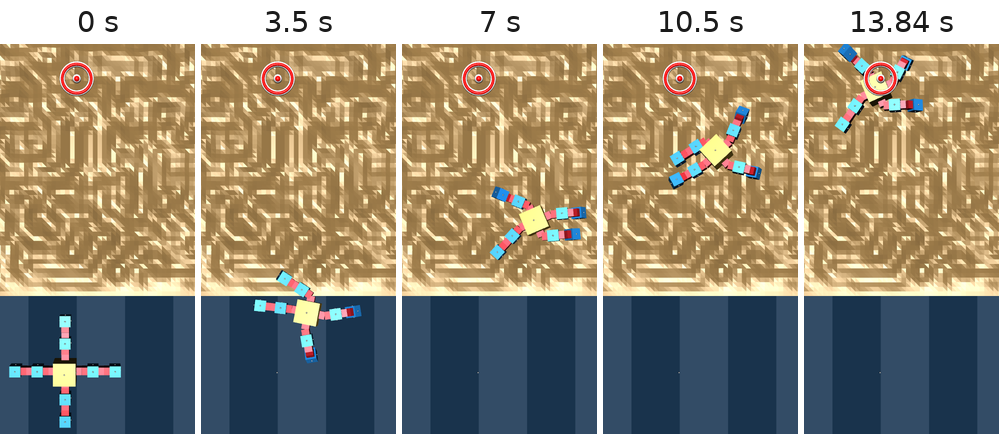
\includegraphics[width=\columnwidth]{figures/walk_filmstrip.png}
  \caption{An evolved brain (standard EA, seed 4) walking up the OlympicArena,
  seen from above, at 0, 4, 8, 12 and 14.3\,s. It starts on the flat part
  (bottom) and reaches the target on the bumpy strip.}
  \label{fig:walk}
\end{figure}

\subsection{Controller}

The controller is a fully connected feed-forward network with two hidden layers
of 8 and 4 \texttt{tanh} neurons and 8 \texttt{tanh} outputs, each scaled to a
target angle in $[-\pi/2, \pi/2]$ for one hinge. With a bias on every neuron it
has 212 weights, which form the genome. Its 16 inputs are listed in
Table~\ref{tab:inputs}. The network has no memory, so it gets a clock to walk
to; the clock is a fixed input signal, not an oscillator inside the controller,
so the controller is not a CPG. The target is given relative to the robot's
heading rather than as an absolute position, so that ``the goal is 1\,m away,
30$^\circ$ to the left'' means the same everywhere on the arena.

\begin{table}[t]
  \caption{The controller's 16 inputs, all scaled to about $[-1, 1]$.}
  \label{tab:inputs}
  \small
  \begin{tabular}{lcl}
    \toprule
    Input & Size & What it tells the controller \\
    \midrule
    Joint angles & 8 & where each hinge is now \\
    Clock & 2 & $\sin$ and $\cos$ of a 1\,Hz beat, for rhythm \\
    Target & 3 & distance / 2\,m; $\sin$, $\cos$ of its bearing \\
    Tilt & 3 & the up direction seen from the core \\
    \bottomrule
  \end{tabular}
\end{table}

\paragraph{Why no vision} Our first controller also had ten distance rays to
the terrain: one down, one up and two per face of the core, so that each side
could ``see'' the ground ahead. They were designed for the rugged world, whose
hills are up to 0.5\,m high. On the OlympicArena only five of them carried
terrain information (the up ray never changed and the four shallow rays mostly
measured the arena's edges), so we kept those five, and then tested three, one
and none against them (three tuning seeds). No smaller set beat five rays on every seed, and no vision tied
with them (0.97 against 0.92\,m from the target on unseen arenas; training
fitness 1.339 against 1.348). Measuring the signals explained why: a ray reads
up to 3\,m while the bumps are about $\pm$2\,cm, so a bump moves a ray input by
less than 0.01, 20--40 times less than the joint angles move, and the rays vary
almost as much on flat ground: they mostly sensed the robot's own bobbing. We
therefore removed vision, which also shrank the genome.

\paragraph{Why 16-8-4-8} Six shapes from 208 to 808 weights were compared on
three seeds (Table~\ref{tab:params}). The bottleneck of four was the only shape
better than our previous single layer of 16 on every seed (mean best fitness
1.203 against 1.339 at 6{,}000 evaluations) and also the best on unseen arenas
(0.85 against 0.97\,m). Driving eight motors through four shared signals pushes
the legs towards coordinated patterns, and halves the number of weights to
search; wider networks were clearly worse at this budget.

\subsection{Fitness function}
\label{sec:fitness}

The assignment's fitness is the planar distance $d_T$ between the core's final
position and the target. We started with exactly that, and nothing walked:
the best networks of our first runs wiggled in place, their joint commands
within $\pm 0.13$ of their range. Penalising the core for touching the ground
and for being upside down made the robots move, but on video they crouched
(the core 1.6\,cm above lying height, although the body can hold it 6\,cm up)
and kept one leg tucked away (5--9$^\circ$ of movement against 17--77$^\circ$
for the other legs). The distance alone gives evolution no reason to walk well
before it walks at all, so we added terms for the mechanics of walking, and
minimise
\begin{equation}
  f = d_T + 0.5\,\bar{d} + 1.0\,c + 1.0\,u + 1.0\,\ell + 0.5\,w ,
  \label{eq:fitness}
\end{equation}
where every term is measured at each 50\,Hz update and lies in $[0, 1]$ except
the distances:
\begin{itemize}
  \item \textbf{Stand} ($c$, $\ell$): $c$ is the share of the walk in which the
  core touches the ground, and $\ell$ is the mean shortfall of the core's lift
  above its lying height from a 4\,cm line, $\mathrm{clip}(1 - \mathrm{lift} /
  4\,\mathrm{cm}, 0, 1)$. The body can hold itself 6\,cm up, so 4\,cm is
  demanding but reachable, and every millimetre up to the line pays.
  \item \textbf{Use all legs alike} ($w$): just as people use both legs about
  equally, each leg should do about a quarter of the work. With $W_i$ the
  positive motor work of leg $i$, $w = 1 - \min_i W_i / \overline{W}$: 0 when
  every leg works alike, 1 when one leg is idle. We first measured how much
  each leg moves, but a leg can move without pushing, and a leg that only props
  the body up carries its share of the weight; only the motor work caught such
  a lazy leg (22\,J against up to 40\,J for the others).
  \item \textbf{Stay upright} ($u$): the share of the walk spent upside down.
  \item \textbf{Be fast} ($\bar d$): the distance to the target averaged over
  the whole 15\,s, counting 0 after arrival, so that closing the distance early,
  and arriving early, lower the fitness.
\end{itemize}
The third mechanic of walking, \textbf{rhythm}, is not a fitness term: it is
provided by the clock input. A robot that holds still scores 5.0 ($d_T = \bar d
= 2$, core on the ground, nothing lifted), and one that arrives at once while
standing tall and using all legs alike scores 0. A typical evolved brain (no
migration, seed 0) scores $0.15 + 0.5 \cdot 1.19 + 0.02 + 0 + 0.18 + 0.5 \cdot
0.19 = 1.04$: the two distance terms dominate, and the gait terms decide
between walkers that get about equally far. This is behavioural shaping: it
prescribes part of \emph{how} to walk, which the assignment allows if the
metric is clearly defined. All conditions use the same fitness, and we report
the plain distance as well.

\subsection{The evolutionary algorithm}

The genome is a fixed-length vector of real numbers, so we use a real-coded
genetic algorithm: Gaussian mutation explores around good weights, and
recombination can combine good neurons found in different individuals. The
island model is both the object of our study and a known guard against
premature convergence on multimodal landscapes.

\paragraph{Representation and variation} A genome is the vector of 212 real
weights, initialised from $\mathcal{N}(0, 0.5^2)$. Parents are chosen by
tournaments of three within an island~\cite{eiben2015introduction}. With probability 0.9 a child is made by
\emph{neuron-level uniform crossover}: for every hidden neuron, a fair coin
decides from which parent it inherits all of that neuron's incoming weights and
bias (the second hidden layer's neurons also take their outgoing weights);
each output bias comes from a random parent. Otherwise the child copies one
parent. Every child is then mutated by adding $\mathcal{N}(0, 0.05^2)$ noise to
every weight, with ARIEL's Gaussian mutation operator. Keeping neurons whole is the
classic response to the competing-conventions problem
\cite{montana1989training,moriarty1996efficient}: the child inherits working
units rather than a mixture of two units that may play different roles.

\paragraph{Survivor selection} Generational with elitism: each island keeps
its two best individuals unchanged and replaces the other 18 by children. As
the arena is fixed, the fitness is deterministic and elites are not
re-evaluated.

\paragraph{Island model} Four islands of 20 individuals form a ring. Every 10
generations each island copies two emigrants to the next island, where they
replace that island's two worst individuals. The emigrant-selection policy is
the variable of the RQ: \emph{best} (the two fittest), \emph{worst} (the two
least fit), \emph{random} (two chosen uniformly) or \emph{none} (no migration,
four isolated islands). Everything else is identical across conditions.

\paragraph{Baselines} The \emph{standard EA} is the same algorithm with one
population of 80 and 8 elites, so only the population structure differs.
\emph{Random search} draws every new genome from the initial distribution and
keeps the best, at the same budget, as the assignment requires.

\paragraph{Budget} Each run stops after 12{,}000 evaluations (80 initial and
72 children per generation: about 166 generations). Instead of a plateau rule,
which never fired before the budget ran out in our pilots, we chose the budget
from where the pilot curves flattened: 95\% of the progress of a long run came
within 5{,}000 evaluations and its last improvement at 8{,}800.

\subsection{How the settings were chosen}

Table~\ref{tab:params} lists every setting with its justification. Settings
were changed by controlled comparisons with a decision rule fixed beforehand:
a new value replaces the current one only if its best fitness after 6{,}000
evaluations is better on all three tuning seeds and on the mean. The tuning
seeds (100--102) and their arenas are disjoint from those of the final
experiment (0--4), and tuning used the random emigrant policy, which favours
none of the policies we compare. The migration interval, the number of
migrants, the topology and the replacement were not tuned: they set the
context of the RQ and take common values from the
literature~\cite{cantupaz2001migration}. Only one tuned value changed:
crossover probability 0.9 (mean best fitness 1.369 against 1.800 at 0.5).
In total the project used 1.87 million evaluations: 0.80 million for
development, 0.53 million for tuning and 0.54 million for the final
experiments.

\begin{table*}[t]
  \caption{Every setting of the final EA and how it was chosen. ``Tested''
  rows were decided by the rule of Section~2.5 (3 seeds, 6{,}000
  evaluations); best fitness shown as the mean over the seeds, lower is
  better.}
  \label{tab:params}
  \small
  \begin{tabularx}{\textwidth}{@{}p{2.6cm}p{4.3cm}X@{}}
    \toprule
    Component & Setting & How it was chosen \\
    \midrule
    Network & 16-8-4-8, \texttt{tanh}, 212 weights & tested against 16-8-8, 16-16-8, 16-32-8, 16-8-8-8, 16-16-16-8: only shape better on every seed (1.203 vs 1.339) \\
    Inputs & 16, no vision & 10 $\to$ 5 rays (pilot); 5 vs 3, 1, 0 rays tested: no difference, rays carry $<$0.01 of signal \\
    Parent selection & tournament, $k = 3$ & $k = 2$ and $5$ tested: inconsistent (1.877, 1.612 vs 1.800) \\
    Crossover & neuron-level uniform & tested against weight-level uniform (1.416), BLX-0.5 (1.168, better on 2 of 3 seeds) and headless chicken (2.207) vs ours (1.203) \\
    Crossover probability & 0.9 & 0, 0.5 and 0.9 tested: 0.9 better on every seed (1.369 vs 1.800; 0 gave 2.063) \\
    Mutation & Gaussian, $\sigma = 0.05$, every weight & pilot over $\sigma \in \{0.05, 0.1, 0.2\}$; then 0.02, 0.1, and 10\% of weights with $\sigma = 0.16$ tested: none better \\
    Mutation-step control & none & a rule doubling $\sigma$ on stagnating islands tested: 1.369 vs 1.348 without, dropped \\
    Survivor selection & generational, 2 elites per island & 1 and 5 elites tested: inconsistent (1.791, 1.811 vs 1.800) \\
    Population & 4 islands $\times$ 20 & $4 \times 10$ and $4 \times 40$ tested: inconsistent (2.020, 1.693) \\
    Migration & ring, every 10 generations, 2 copies, replace worst & literature~\cite{cantupaz2001migration}; not tuned (context of the RQ); interval studied afterwards (Section~4.3) \\
    Budget & 12{,}000 evaluations ($\approx$166 generations) & pilot curves: 95\% of the progress by 5{,}000, last gain at 8{,}800 \\
    Walk & 15\,s, ends at the target & the template's length; 20\,s training walks tested: no better on unseen arenas \\
    \bottomrule
  \end{tabularx}
\end{table*}

% =====================================================================
\section{Experimental setup}
\label{sec:setup}

\paragraph{Conditions} Six conditions: the island EA with the \emph{best},
\emph{worst}, \emph{random} and \emph{none} policies, the standard EA and
random search. Each runs on seeds 0--4; a seed fixes the EA's random numbers
and the arena, and all conditions with the same seed share that arena, which
pairs the runs.

\paragraph{Metrics} Lower is better for all.
(1)~The best-so-far fitness against evaluations, and its area under the curve
(AUC), which rewards being good early.
(2)~Convergence speed: the evaluations until the best fitness first drops below
1.6. This threshold separated fast from slow runs in tuning, where no untuned
run reached it.
(3)~The final best fitness after 12{,}000 evaluations, and the closest any
brain got to the target.
(4)~Generalisation: each run's best brain walks 20 fresh arenas it never saw,
and we report the mean distance left.

\paragraph{Statistics} A Friedman test across the six conditions, blocked by
seed, asks whether they differ at all; planned two-sided Mann--Whitney tests
against \emph{none} with Holm's correction ask which do. With five seeds the
smallest attainable $p$ is 0.008, so only large effects can be significant. We
therefore also report, for every pair of conditions, the probability that one
has the lower true mean, from a Bayesian paired $t$-test with a flat
prior~\cite{benavoli2017time}, with differences within $\pm0.05$ counting as
practically equal, and the Vargha--Delaney $A_{12}$ effect
size~\cite{vargha2000critique}.

\paragraph{Follow-ups} (a) The migration interval: the \emph{best} policy
migrating every 5, 20 and 50 generations, on the same seeds and arenas; the
main experiment supplies every 10 and never. (b) Longer test walks: every best
brain walks its own arena for 15, 20, 30 and 60\,s and the unseen arenas for
30\,s, to see whether the 15\,s limit or the gait stops the robots.

\paragraph{Reproducibility} The code builds on ARIEL without changing it; one
script per experiment runs all seeds of all conditions. A run takes about 10
minutes on an Apple M3 Pro with 10 worker processes; the 45 final runs took
6.4 hours. \todo{name the scripts or the repository in one sentence}

% =====================================================================
\section{Results}

\subsection{Convergence and final fitness}

\begin{figure*}[t]
  \centering
  \maybegraphic{\textwidth}{figures/convergence.pdf}
  \caption{Best-so-far fitness (a) and closest distance to the target (b)
  against generations (top axis: evaluations), for every condition: the mean
  over 5 seeds, with a band of $\pm 1$ standard deviation. Lower is better.}
  \label{fig:convergence}
\end{figure*}

\begin{table*}[t]
  \caption{Results after 12{,}000 evaluations, mean $\pm$ standard deviation
  over 5 seeds (lower is better). ``Closest'' is the closest any brain of the
  run got to the target; ``to 1.6'' counts only the runs that got there.
  P(faster) is the posterior probability that the condition has a lower AUC
  than no migration.}
  \label{tab:results}
  \small
  \begin{tabular}{lcccccc}
    \toprule
    Condition & Final fitness & Closest (m) & Evaluations to 1.6 & AUC & Unseen arenas (m) & P(faster than none) \\
    \midrule
    Migrate best   & 1.130 $\pm$ 0.317 & 0.296 $\pm$ 0.227 & \textbf{2{,}906 $\pm$ 364} (4/5) & 1.491 $\pm$ 0.218 & 0.857 $\pm$ 0.250 & 96\% \\
    Migrate worst  & 1.172 $\pm$ 0.277 & 0.313 $\pm$ 0.165 & 4{,}976 $\pm$ 2{,}626 (5/5) & 1.582 $\pm$ 0.226 & \textbf{0.830 $\pm$ 0.178} & 94\% \\
    Migrate random & 1.137 $\pm$ 0.217 & 0.279 $\pm$ 0.173 & 4{,}846 $\pm$ 1{,}797 (5/5) & 1.545 $\pm$ 0.224 & 0.863 $\pm$ 0.078 & 89\% \\
    No migration   & 1.245 $\pm$ 0.211 & 0.390 $\pm$ 0.190 & 5{,}466 $\pm$ 2{,}329 (5/5) & 1.649 $\pm$ 0.164 & 0.911 $\pm$ 0.156 & -- \\
    Standard EA    & \textbf{0.957 $\pm$ 0.252} & \textbf{0.225 $\pm$ 0.157} & 3{,}190 $\pm$ 1{,}436 (5/5) & \textbf{1.431 $\pm$ 0.207} & 0.885 $\pm$ 0.107 & 90\% \\
    Random search  & 2.603 $\pm$ 0.110 & 1.322 $\pm$ 0.052 & never (0/5) & 2.681 $\pm$ 0.072 & 1.454 $\pm$ 0.108 & 0\% \\
    \bottomrule
  \end{tabular}
\end{table*}

Figure~\ref{fig:convergence} and Table~\ref{tab:results} summarise the main
experiment. Every EA beats random search by a wide margin (Friedman
$\chi^2 = 13.0$, $p = 0.023$; random search against no migration, Holm-corrected
$p = 0.04$; posterior probability 100\% for every EA). Random search never
reached a fitness of 1.6 and ended 1.32\,m from the target.

The policies differ in \emph{speed}. Migrating the best reached fitness 1.6
after $2{,}906 \pm 364$ evaluations, the other policies after about 4{,}900
and the isolated islands after $5{,}466 \pm 2{,}329$. Measured by the AUC,
every migration policy is faster than no migration with posterior probability
89--96\%, and migrating the best is faster than migrating the worst (88\%) or
random individuals (68\%). The policies hardly differ in the \emph{outcome}:
after 12{,}000 evaluations best and random are practically tied (1.130 against
1.137; 52\%), and both are probably, but far from certainly, better than no
migration (73\% and 84\%; e.g.\ best minus none $-0.115$, 95\% interval
$-0.580$ to $+0.351$). None of the planned frequentist comparisons between EAs
is significant. Unexpectedly, the standard EA ended best ($0.957 \pm 0.252$;
78--94\% better than each island variant) and was about as fast as migrating
the best (AUC 65\% in its favour). Figure~\ref{fig:probabilities} shows every
pairwise comparison of convergence speed.

\begin{figure}[t]
  \centering
  \maybegraphic{\columnwidth}{figures/probabilities.pdf}
  \caption{Probability that the row condition converges faster (has a lower
  AUC) than the column condition, from a Bayesian paired $t$-test over the 5
  seeds. Blue: the row is probably faster; orange: probably slower.}
  \label{fig:probabilities}
\end{figure}

\subsection{What the fitness rewards}

\begin{figure}[t]
  \centering
  \maybegraphic{\columnwidth}{figures/fitness_terms.pdf}
  \caption{The final champions' fitness split into the weighted terms of
  Equation~\ref{eq:fitness}, mean over 5 seeds; ``mean distance'' is
  $0.5\,\bar d$. No champion was ever upside down.}
  \label{fig:terms}
\end{figure}

Figure~\ref{fig:terms} splits the champions' fitness into its terms. The speed
term $0.5\,\bar d$ is the largest part of every EA's champion, about half of
its fitness, and larger than the final distance. The gait terms add only
0.20--0.27 together: no champion is ever upside down and the core hardly
touches the ground ($c \leq 0.02$), so the remaining gait differences come from
body height and work balance. The posture terms shaped the gait early in
evolution and then left the ranking to the distance terms.

\subsection{Generalisation to unseen arenas}

On their own arena the best brains end 0.23--0.39\,m from the target; on 20
unseen arenas they end 0.83--0.91\,m away, whatever the policy
(Table~\ref{tab:results}). The differences between the EAs there are
practically zero: for best against worst, 61\% of the posterior lies within
$\pm 0.05$\,m. All evolved brains specialise to the arena they were trained
on.

\subsection{Follow-up: how often to migrate}

\begin{figure}[t]
  \centering
  \maybegraphic{\columnwidth}{figures/interval.pdf}
  \caption{The \emph{best} policy migrating every 5, 10, 20 or 50
  generations, or never (``off''), 5 seeds each. (a) Final best fitness and
  (b) distance left on 20 unseen arenas: dots are seeds, black the mean with
  its 95\% interval. (c) Share of generations in which all four islands hold
  the same champion; dots are seeds.}
  \label{fig:interval}
\end{figure}

Figure~\ref{fig:interval} shows a clear sweet spot. Migrating every 5, 10 or 20
generations is equally fast (AUC probabilities 42--58\% between them), and all
three are faster than every 50 generations (93--99\%) or never (96--100\%).
Three migrations in 166 generations are too few to matter: every 50 is as slow
as no migration. The more often the best migrate, the sooner one champion
occupies all islands: in 35\% of generations at every 5, against 6\% at every
20. Every 20 generations kept the islands apart and still had the best final
fitness (1.093) and the best result on unseen arenas (0.76\,m; 77\% better
than every 10, 99\% than never).

\subsection{Follow-up: is 15 seconds enough?}

\begin{table}[t]
  \caption{Best brains that reach their own target when walking longer, of 30
  (5 seeds $\times$ 6 conditions), and the share of unseen-arena walks that
  reach it.}
  \label{tab:longer}
  \small
  \begin{tabular}{lcccc}
    \toprule
    Walk length & 15\,s (training) & 20\,s & 30\,s & 60\,s \\
    \midrule
    Own arena & 3 & 11 & 11 & 12 \\
    Unseen arenas & 0--4\% & -- & 5--13\% & -- \\
    \bottomrule
  \end{tabular}
\end{table}

\begin{figure}[t]
  \centering
  \maybegraphic{\columnwidth}{figures/longer_walks.pdf}
  \caption{Trained on 15\,s walks, tested for 15\,s (open) and 30\,s (filled).
  (a) Best brains that reach the target on their own arena, of 5 per
  condition. (b) Share of the walks on 20 unseen arenas that reach it.}
  \label{fig:longer}
\end{figure}

Only 3 of the 30 best brains reach the target within the 15\,s they were
trained for (Table~\ref{tab:longer}, Figure~\ref{fig:longer}). Given 20\,s,
eight more arrive, between 15.2 and 19.6\,s: they head for the target and run
out of time. The others stall 0.2--0.7\,m away, legs still moving but the body
no longer advancing, and more time does not help (one more arrives within
60\,s). On unseen arenas, 30\,s instead of 15\,s raises the share of walks
that arrive from 0--4\% to 5--13\%; generalisation remains the main limit.
Random search never arrives, and the policy hardly matters here either (1--3
of 5 brains per EA at 30\,s).

% =====================================================================
\section{Discussion}

\paragraph{Answer to the RQ} The emigrant-selection policy changes how fast
the islands improve but not where they end. H1 is supported: any migration
beats isolated islands on convergence speed (89--96\%). H2 is half supported:
migrating the best is the fastest, as the selection-pressure argument
predicts~\cite{cantupaz2001migration}, but within our budget it does not end
at a worse plateau than random migration; the two tie. H3 is rejected:
migrating the worst still speeds up the islands nearly as much as random
migration (94\% faster than none).

\paragraph{Why migrating the worst helps} In a generational EA with two
elites per island, an island's worst individuals are not random genomes: they
are fresh children of tournament-selected parents, carrying the source
island's working neurons. With a crossover probability of 0.9, the receiving
island recombines these neurons with its own, so even the worst emigrants
inject useful diversity. Moreover, every policy replaces the receiver's worst
individuals, so even the worst emigrants only displace natives that are no
better.

\paragraph{Diversity against speed} Migrating the best quickly copies one
champion around the ring: at every 10 generations all four islands share it
in 28\% of the generations, from about 6{,}800 evaluations on. That explains
its speed, and the follow-up shows the cost: migrating less often (every 20)
kept the islands different and gave the best final and unseen results, while
migrating too rarely (every 50) wasted the islands entirely. Within this
design, the interval is the stronger lever; the policy decides mainly how fast
good genes spread.

\paragraph{Why one population did as well} Islands trade speed for diversity
that pays off in long runs on deceptive problems. Our budget is short (166
generations) and the panmictic population keeps the 8 best individuals
overall, where the islands keep the 2 best of each island, some of which are
worse. Exploitation wins at this budget; a longer run might reverse the order.
\todo{decide whether to test this or leave it as future work}

\paragraph{Limitations} Five seeds give wide intervals: most differences
between policies are probable rather than certain, and none is significant by
a classical test. The settings were tuned with one factor at a time on three
seeds, which misses interactions~\cite{eiben2011parameter}, and with the
random policy, so they may suit the policies unevenly. The fitness shapes the
gait (Section~\ref{sec:fitness}), so ``better'' means better by our definition;
the plain distance gives nearly the same ordering (Table~\ref{tab:results}). Brains
specialise to their arena, a single body and world were used, and the 15\,s
limit stops a third of the brains that would arrive. Training on three arenas
with turned starts, or with 20\,s walks, did not improve generalisation in a
pilot at 6{,}000 evaluations~\cite{jakobi1997evolutionary}; it may need a
larger budget.

% =====================================================================
\section{Conclusion}

We evolved neural controllers that make \texttt{spider\_8} walk to a target
2\,m away and asked whom an island model should send between its islands.
Migration of any kind speeds up evolution compared with isolated islands, and
migrating the best is the fastest, reaching a fitness of 1.6 in about half the
evaluations of isolated islands. The final controllers and their behaviour on
unseen arenas do not depend measurably on the policy, and a single population
did as well at our budget. How often the islands migrate matters more:
every 5--20 generations is equally fast, every 50 is as slow as never, and
every 20 kept the islands most diverse. Future work: longer budgets, where the
diversity islands preserve should pay off; more seeds; recombination that
aligns an immigrant's neurons with the natives' before
crossing~\cite{uriot2020safe}; and training that varies the arena enough for
the controllers to generalise. These conclusions rest on five seeds, one body,
one world and a fitness that shapes the gait.

\bibliographystyle{ACM-Reference-Format}
\bibliography{references}

% The course asks every member to list their own contributions at the end.
\section*{Contributions}
\todo{each member: one or two lines on what they did}

\end{document}
